\clearpage

\section{Data vs. MC Comparison in Preselection Region}
\label{sec:yields}

In this section we compare the data and MC samples passing the selection described in Sec.~\ref{sec:eventSelection}
In the following, the MC is reweighted to match the data distribution of number of reconstructed primary vertices.
The trigger efficiencies of Sec.~\ref{sec:datasets} are applied. In all plots, the last bin contains the overflow.
Note that we show here data vs. MC comparisons as a sanity check only, since the dominant backgrounds estimated from data.

We begin by counting the inclusive Z yields. Here we require the presence of two selected leptons without
any additional requirements on jets or \MET. In Fig.~\ref{fig:dilmass} the distribution of dilepton invariant
mass in the ee and $\mu\mu$ channels is displayed. In Table~\ref{table:zyields} the yields for selected dilepton
events in the Z mass window are indicated. Good data vs. MC agreement is observed, within the systematic uncertainties
of integrated luminosity (4.5\%), trigger efficiency (3\%), \zjets\ and \ttbar\ cross sections.

\begin{figure}[hbt]
  \begin{center}
	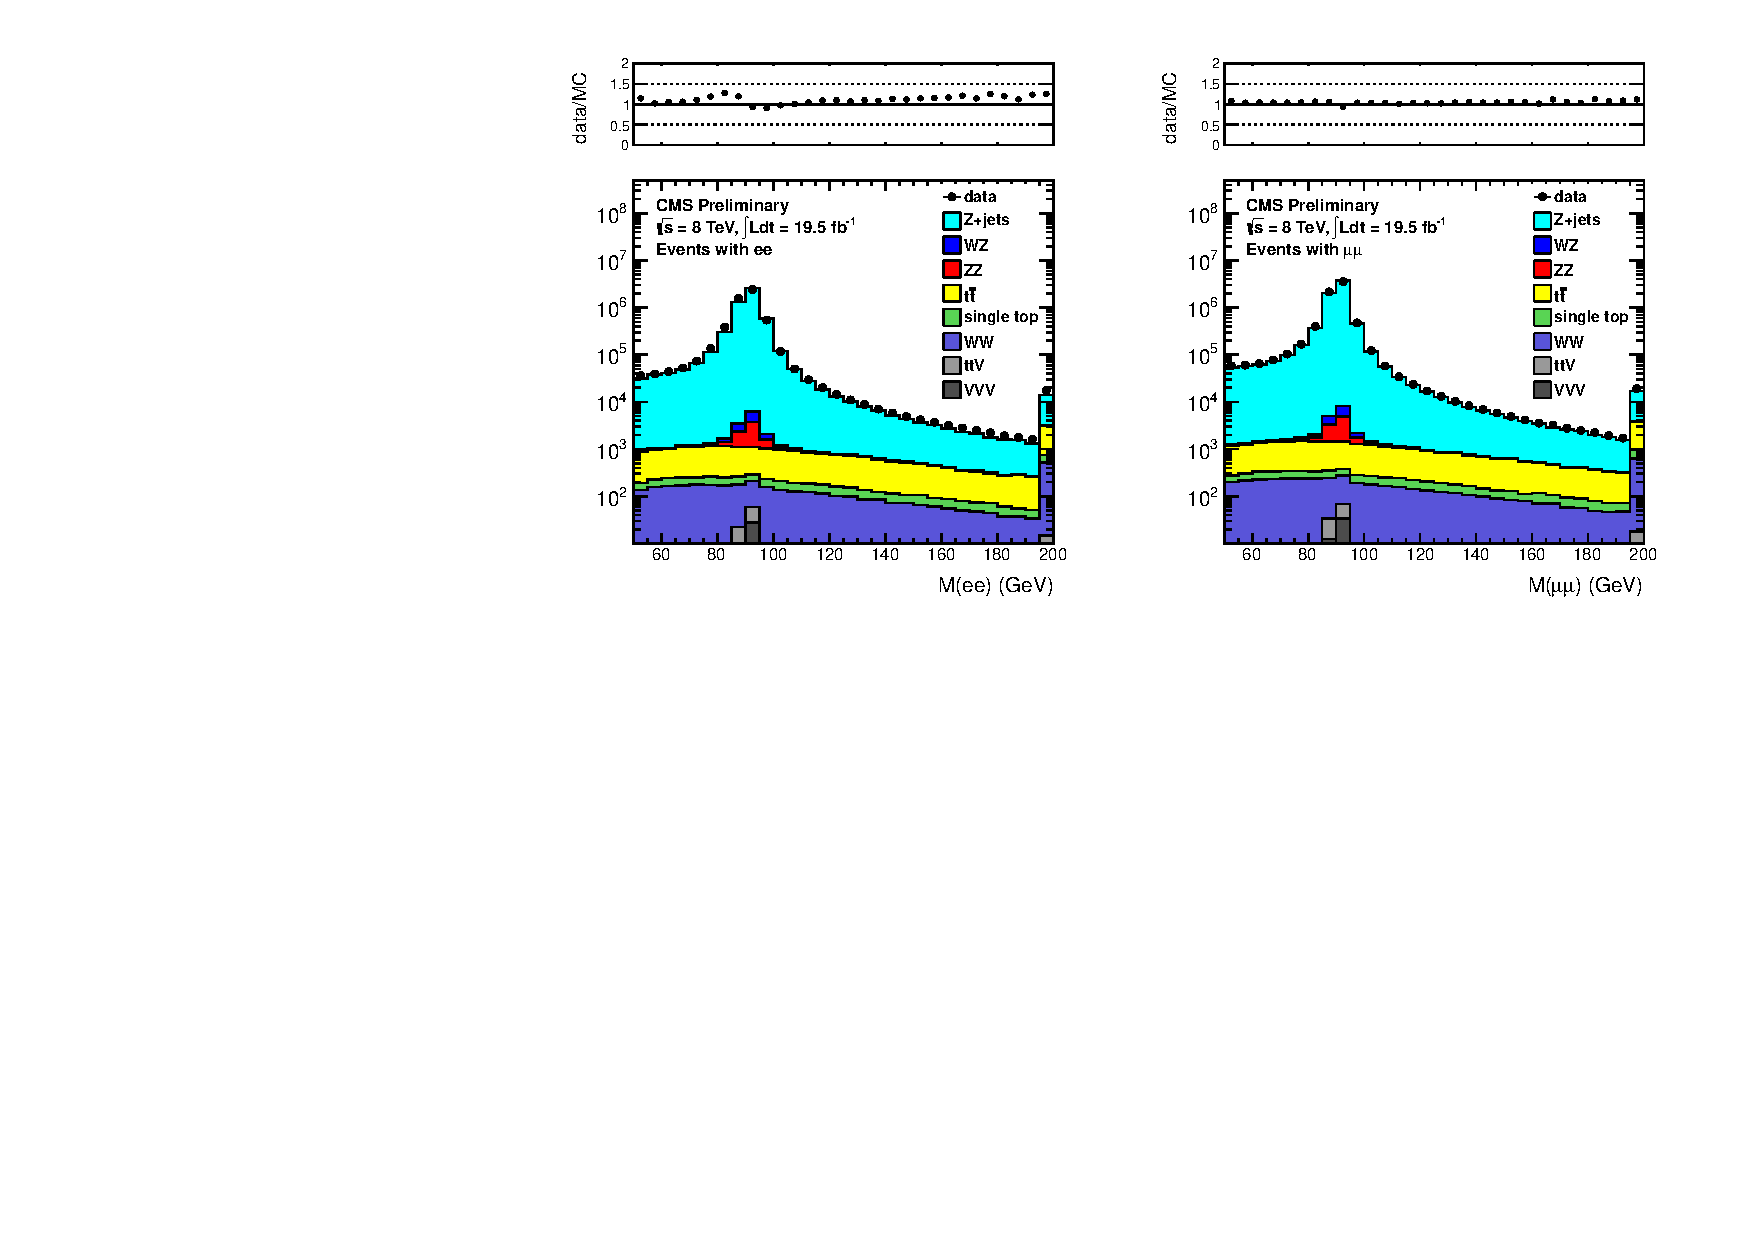
\includegraphics[width=1.0\linewidth]{plots/dilmass_19p5fb.pdf}
	\caption{
	  \label{fig:dilmass}\protect 
	  Dilepton mass distribution for events with two selected leptons
	  in the ee (left) and $\mu\mu$ (right) final states.}

%Loading babies at       : ../output/V00-02-13
%Using selection         : (((((leptype==0 && (ee==1 || isdata==0))||(leptype==1 && (mm==1 || isdata==0)))||(leptype==2 && (em==1||me==1||isdata==0)))&&(csc==0 && hbhe==1 && hcallaser==1 && ecaltp==1 && trkfail==1 && eebadsc==1 && hbhenew==1))&&(lep1.pt()>20.0 && lep2.pt()>20.0))&&(dilmass>15.0)
%Using weight            : weight * 19.5 * trgeff * vtxweight
%Plotting var dilmass flavor ee
%compareDataMC : apply trigeff 1
%MC yield VVV 46.80
%MC yield ttV 110.19
%MC yield WW 3487.10
%MC yield single top 1798.02
%MC yield ttbar 18784.90
%MC yield ZZ 5335.59
%MC yield WZ 5014.99
%MC yield zjets 5412155.17
%MC total yield 5446733.00
%data yield 5.60839e+06
%Plotting var dilmass flavor mm
%compareDataMC : apply trigeff 1
%Warning in <TROOT::Append>: Replacing existing TH1: htemp (Potential memory leak).
%MC yield VVV 55.66
%MC yield ttV 130.83
%MC yield WW 4360.91
%MC yield single top 2219.78
%MC yield ttbar 22376.46
%MC yield ZZ 6658.82
%MC yield WZ 6187.59
%MC yield zjets 7012986.51
%MC total yield 7054976.50
%data yield 7.44544e+06

  \end{center}
\end{figure}


\begin{table}[htb]
\begin{center}
\caption{\label{table:zyields} Data and Monte Carlo yields for events with two selected leptons in the Z mass window. }
\begin{tabular}{lccccc}

%Loading babies at       : ../output/V00-02-13
%Using selection         : ((((((leptype==0 && (ee==1 || isdata==0))||(leptype==1 && (mm==1 || isdata==0)))||(leptype==2 && (em==1||me==1||isdata==0)))&&(csc==0 && hbhe==1 && hcallaser==1 && ecaltp==1 && trkfail==1 && eebadsc==1 && hbhenew==1))&&(lep1.pt()>20.0 && lep2.pt()>20.0))&&(dilmass>15.0))&&(dilmass>81 && dilmass<101)
%Using weight            : weight * 19.5 * trgeff * vtxweight

\hline
\hline
         Sample   &             ee   &       $\mu\mu$   &         e$\mu$   &          total  \\
\hline
         \zjets   &4776593 $\pm$ 3391   &6227613 $\pm$ 3627   &2328 $\pm$ 73.9   &11006533 $\pm$ 4966  \\
         \ttbar   &3321.1 $\pm$ 45.8        &4014.4 $\pm$ 47.6        &7621.3 $\pm$ 68.7   &14956.8 $\pm$ 95.3  \\
             WW   &614.8 $\pm$ 6.0          &773.7 $\pm$ 6.3          &1433.1 $\pm$ 9.0    &2821.7 $\pm$ 12.6  \\
             WZ   &4342.7 $\pm$ 7.3         &5411.7 $\pm$ 7.7         &115.3 $\pm$ 1.1     &9869.7 $\pm$ 10.6  \\
             ZZ   &4712.8 $\pm$ 9.9         &5906.1 $\pm$ 10.5        & 21.0 $\pm$ 0.3     &10639.8 $\pm$ 14.4  \\
     single top   &315.3 $\pm$ 11.9         &388.4 $\pm$ 12.4         &709.5 $\pm$ 17.6    &1413.2 $\pm$ 24.6  \\
           \ttV   & 57.4 $\pm$ 1.1          & 68.1 $\pm$ 1.1          & 21.8 $\pm$ 0.7     &147.3 $\pm$ 1.7  \\
            VVV   & 30.1 $\pm$ 0.3          & 36.4 $\pm$ 0.4          &  6.9 $\pm$ 0.2     & 73.5 $\pm$ 0.5  \\
\hline
    total SM MC   &4789987.0 $\pm$ 3391.1   &6244211.0 $\pm$ 3627.1   &12256.7 $\pm$ 102.8   &11046454.7 $\pm$ 4966.5  \\
\hline
           data   &        4906970   &        6552612   &          13141   &       11472723  \\
\hline
\hline

\end{tabular}
\end{center}
\end{table}

\clearpage

We next define the preselection region for the inclusive search using the following requirements:
\begin{itemize}
\item Number of jets $\geq$ 2;
\item Same flavor dileptons (opposite flavor yields will be shown since they are used in data for the FS background estimation);
\item Dilepton invariant mass $81<m_{\ell\ell}<101$ GeV.
\end{itemize}

The dilepton mass distributions in the preselection region of the inclusive search (without the dilepton mass requirement applied) 
for the ee and $\mu\mu$ final states are shown in Figure~\ref{fig:dilmass_2j}. In Table~\ref{table:zyields_2j} the data and MC yields 
in the inclusive preselection region are indicated. Good data vs. MC agreement is observed.


\begin{figure}[hbt]
  \begin{center}
	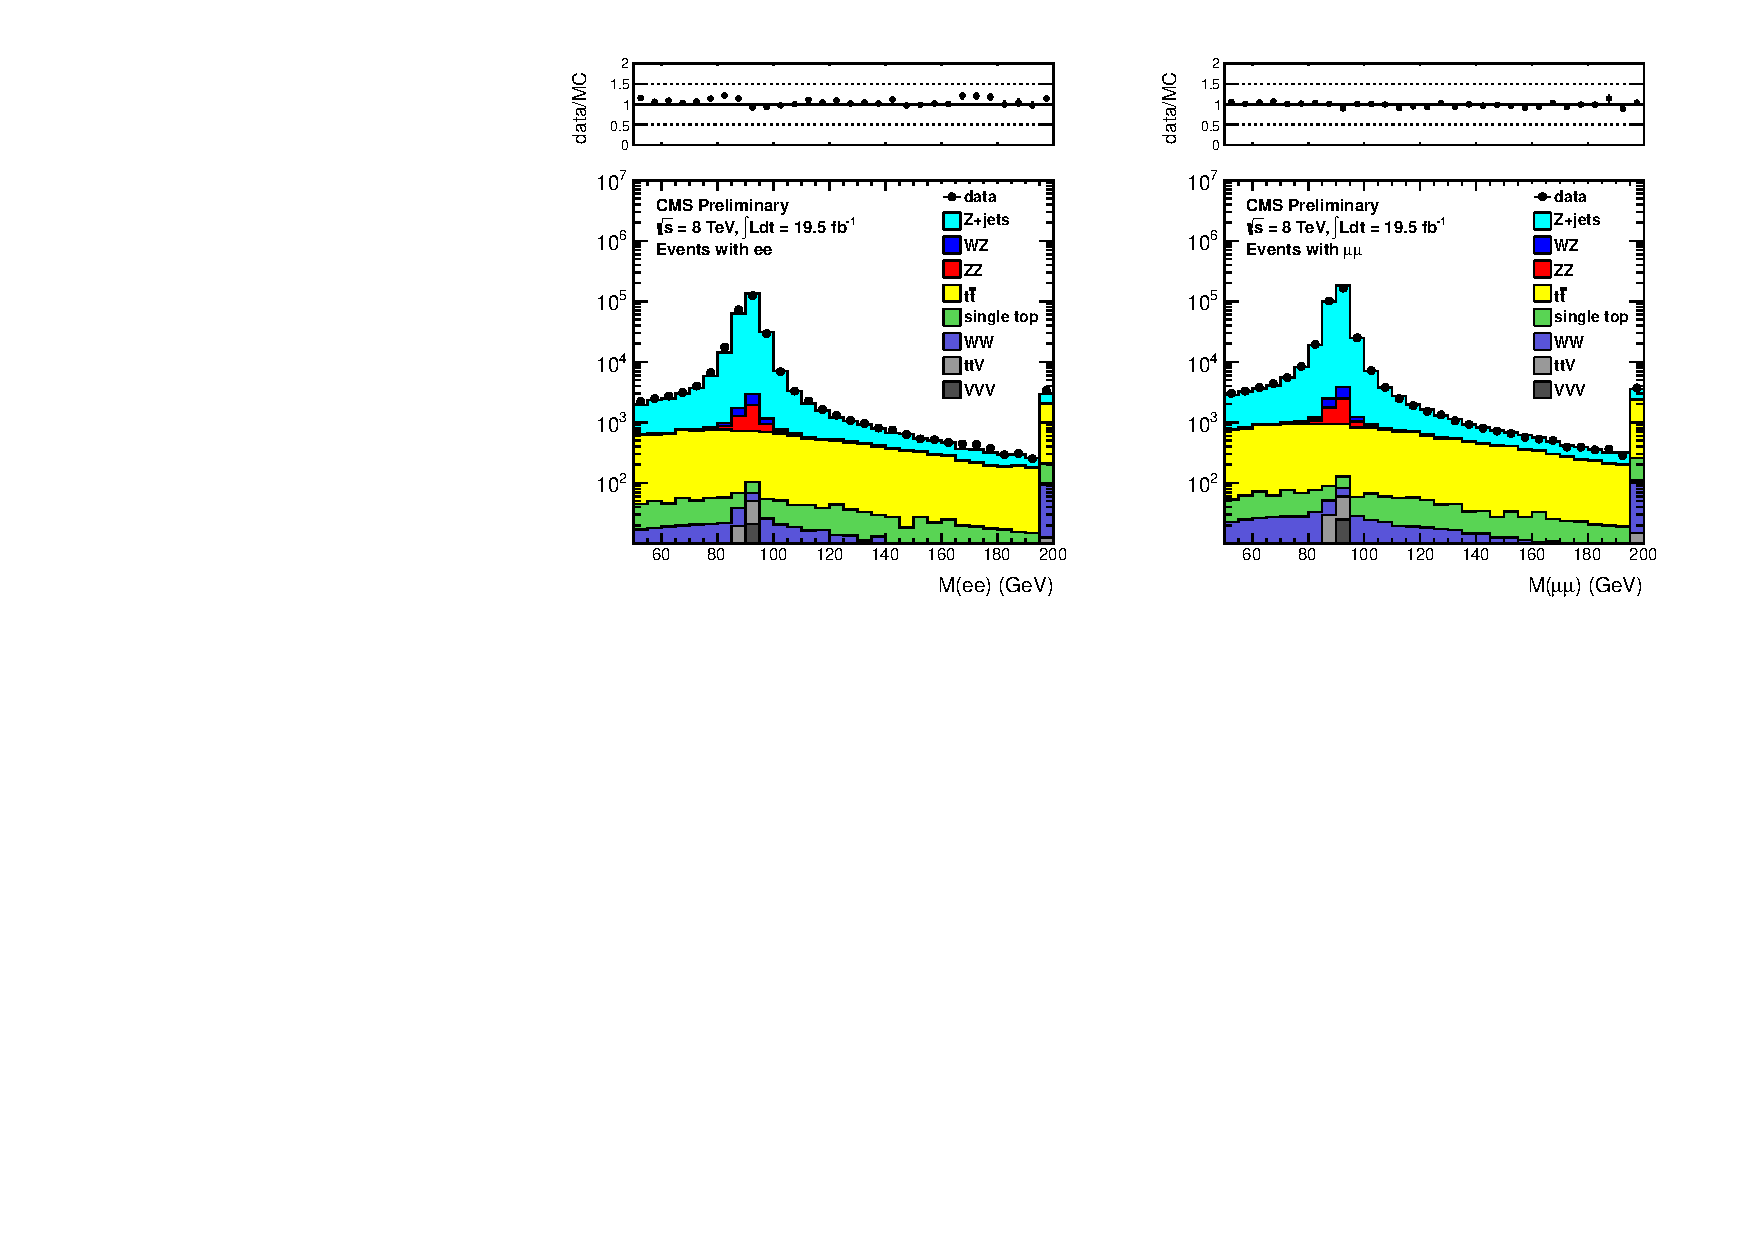
\includegraphics[width=1.0\linewidth]{plots/dilmass_2jets_19p5fb.pdf}
	\caption{
	  \label{fig:dilmass_2j}\protect 
	  Dilepton mass distribution for events in the preselection region of the inclusive search
	  in the ee (left) and $\mu\mu$ (right) final states.}

%Loading babies at       : ../output/V00-02-13
%-------------------------------------
%USING SKIMMED SAMPLES WITH NJETS >= 2
%-------------------------------------

%Using selection         : ((((((leptype==0 && (ee==1 || isdata==0))||(leptype==1 && (mm==1 || isdata==0)))||(leptype==2 && (em==1||me==1||isdata==0)))&&(csc==0 && hbhe==1 && hcallaser==1 && ecaltp==1 && trkfail==1 && eebadsc==1 && hbhenew==1))&&(lep1.pt()>20.0 && lep2.pt()>20.0))&&(dilmass>15.0))&&(njets>=2)
%Using weight            : weight * 19.5 * trgeff * vtxweight
%Plotting var dilmass flavor ee
%compareDataMC : apply trigeff 1
%MC yield VVV 31.28
%MC yield ttV 103.46
%MC yield WW 366.01
%MC yield single top 722.28
%MC yield ttbar 14229.66
%MC yield ZZ 2258.35
%MC yield WZ 1956.41
%MC yield zjets 196280.15
%MC total yield 215947.61
%data yield 224358
%Plotting var dilmass flavor mm
%compareDataMC : apply trigeff 1
%Warning in <TROOT::Append>: Replacing existing TH1: htemp (Potential memory leak).
%MC yield VVV 37.07
%MC yield ttV 123.73
%MC yield WW 444.00
%MC yield single top 881.50
%MC yield ttbar 16957.57
%MC yield ZZ 2782.22
%MC yield WZ 2384.37
%MC yield zjets 246103.06
%MC total yield 269713.53
%data yield 281148

  \end{center}
\end{figure}

\begin{table}[htb]
\begin{center}
\caption{\label{table:zyields_2j} Data and MC yields in the preselection region of the inclusive search.
}
\begin{tabular}{lccccc}

%Loading babies at       : ../output/V00-02-13
%-------------------------------------
%USING SKIMMED SAMPLES WITH NJETS >= 2
%-------------------------------------

%Using selection         : (((((((leptype==0 && (ee==1 || isdata==0))||(leptype==1 && (mm==1 || isdata==0)))||(leptype==2 && (em==1||me==1||isdata==0)))&&(csc==0 && hbhe==1 && hcallaser==1 && ecaltp==1 && trkfail==1 && eebadsc==1 && hbhenew==1))&&(lep1.pt()>20.0 && lep2.pt()>20.0))&&(dilmass>15.0))&&(njets>=2))&&(dilmass>81 && dilmass<101)
%Using weight            : weight * 19.5 * trgeff * vtxweight

\hline
\hline
         Sample   &             ee   &       $\mu\mu$   &         e$\mu$   &          total  \\
\hline
         \zjets   &174022.4 $\pm$ 645.0   &218277.0 $\pm$ 678.9   &86.9 $\pm$ 14.4   &392386.4 $\pm$ 936.5  \\
         \ttbar   &2536.3 $\pm$ 40.1   &3058.7 $\pm$ 41.6   &5824.7 $\pm$ 60.1   &11419.7 $\pm$ 83.3  \\
             WW   & 59.5 $\pm$ 1.9   & 73.2 $\pm$ 1.9   &134.2 $\pm$ 2.8   &266.9 $\pm$ 3.9  \\
             WZ   &1709.7 $\pm$ 4.7   &2098.1 $\pm$ 4.9   & 20.0 $\pm$ 0.4   &3827.8 $\pm$ 6.8  \\
             ZZ   &2002.4 $\pm$ 6.9   &2477.2 $\pm$ 7.2   &  4.2 $\pm$ 0.2   &4483.8 $\pm$ 9.9  \\
     single top   &121.2 $\pm$ 7.4   &137.7 $\pm$ 7.4   &263.7 $\pm$ 10.7   &522.6 $\pm$ 15.0  \\
           \ttV   & 54.9 $\pm$ 1.0   & 65.6 $\pm$ 1.1   & 20.0 $\pm$ 0.6   &140.5 $\pm$ 1.6  \\
            VVV   & 21.7 $\pm$ 0.3   & 26.2 $\pm$ 0.3   &  3.4 $\pm$ 0.1   & 51.3 $\pm$ 0.4  \\
\hline
    total SM MC   &180528.1 $\pm$ 646.4   &226213.8 $\pm$ 680.2   &6357.1 $\pm$ 62.7   &413098.9 $\pm$ 940.4  \\
\hline
           data   &         185555   &         234132   &           6231   &         425918  \\
\hline
\hline

\end{tabular}
\end{center}
\end{table}


\clearpage

We next define the preselection region for the targeted search by adding the following requirements:
\begin{itemize}
\item Veto events containing a b-tagged jet;
\item Dijet invariant mass $70<m_{jj}<110$ GeV;
\item Veto events containing a third selected lepton (electron or muon) with \pt $>$ 10 GeV; 
\end{itemize}

The rejection of events with a b-tagged jet strongly suppresses the \ttbar\ background, which is the dominant background in the inclusive search
after requiring large \MET. The requirement that the jet pair is consistent with originating from W/Z decay is motivated by the fact that we are 
searching for signatures producing V(jj)Z($\ell\ell$)+\MET; this requirement suppresses the \zjets\ and \ttbar\ backgrounds. The veto of events
containting a third electron or muon suppresses the WZ background, and also serves to make this analyis exclusive with respect to searches in
the trilepton final state.

The dilepton mass distributions in the preselection region of the targeted search (without the dilepton mass requirement applied) 
for the ee and $\mu\mu$ final states are shown in Figure~\ref{fig:dilmass_2j_targeted}. In Table~\ref{table:zyields_2j_targeted} 
the data and MC yields in the preselection region are indicated. Good data vs. MC agreement is observed.
We also show the distribution of dijet mass in the targeted preselection (with the requirement on this quantity removed) in Fig.~\ref{fig:mjj},
which demonstrates that the MC does a reasonable job of modeling this quantity. The dijet mass selection efficiency for data and MC
is quantified in Table~\ref{table:mjj}. Data/MC comparison of the dilepton \pt\ are shown in Fig.~\ref{fig:zpt}.

%-------------------------------------
% veto b-jets with CSV MEDIUM 
%-------------------------------------

\begin{figure}[hbt]
  \begin{center}
	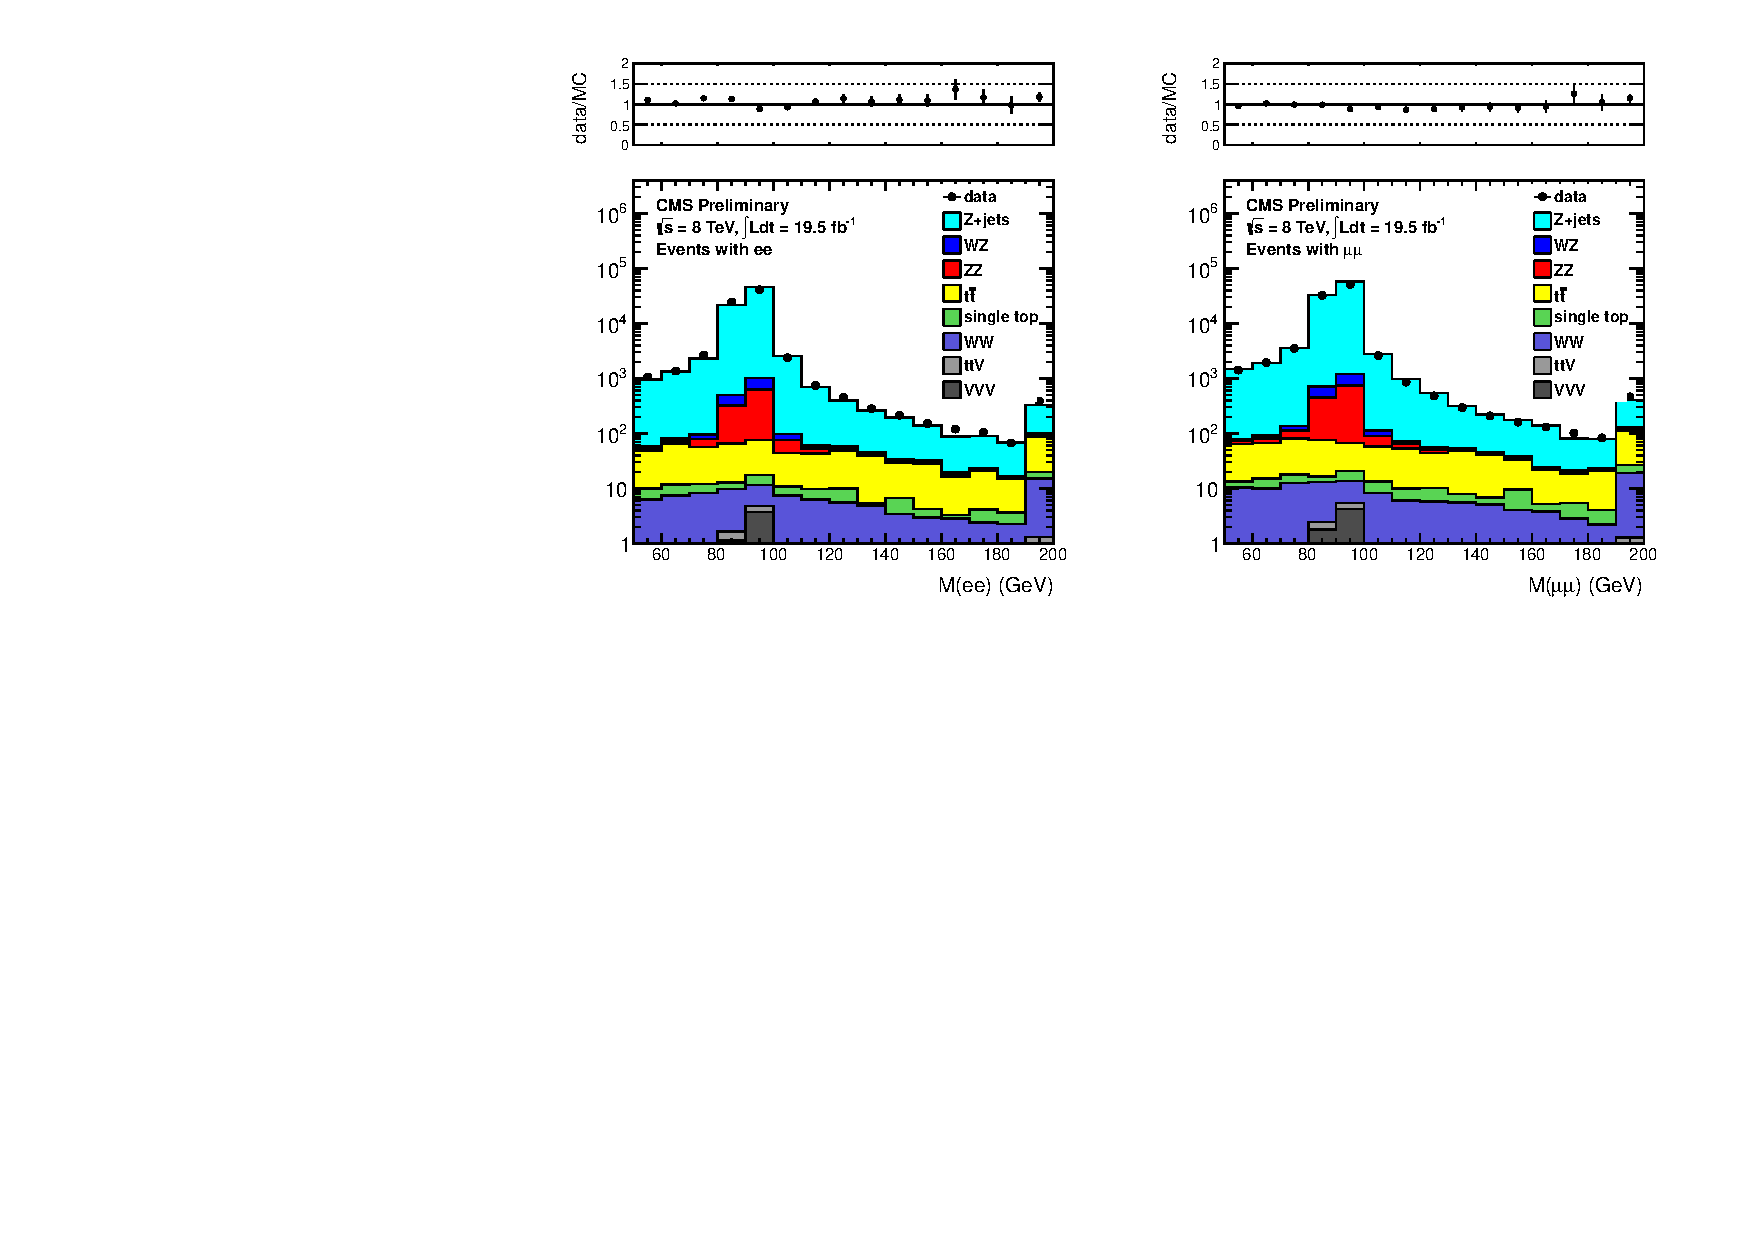
\includegraphics[width=1.0\linewidth]{plots/dilmass_targeted_19p5fb.pdf}
	\caption{
	  \label{fig:dilmass_2j_targeted}\protect 
	  Dilepton mass distribution for events in the preselection region of the targeted search
	  in the ee (left) and $\mu\mu$ (right) final states.}

%Loading babies at       : ../output/V00-02-13
%-------------------------------------
%USING SKIMMED SAMPLES WITH NJETS >= 2
%-------------------------------------

%Using selection         : (((((((((leptype==0 && (ee==1 || isdata==0))||(leptype==1 && (mm==1 || isdata==0)))||(leptype==2 && (em==1||me==1||isdata==0)))&&(csc==0 && hbhe==1 && hcallaser==1 && ecaltp==1 && trkfail==1 && eebadsc==1 && hbhenew==1))&&(lep1.pt()>20.0 && lep2.pt()>20.0))&&(dilmass>15.0))&&(njets>=2))&&(nbcsvm==0))&&(mjj>70.0 && mjj<110.0))&&(nlep==2)
%Using weight            : weight * 19.5 * trgeff * vtxweight
%Plotting var dilmass flavor ee
%compareDataMC : apply trigeff 1
%MC yield VVV 5.81
%MC yield ttV 3.52
%MC yield WW 65.58
%MC yield single top 39.09
%MC yield ttbar 515.71
%MC yield ZZ 876.67
%MC yield WZ 597.84
%MC yield zjets 47170.90
%MC total yield 49275.13
%data yield 50069
%Plotting var dilmass flavor mm
%compareDataMC : apply trigeff 1
%Warning in <TROOT::Append>: Replacing existing TH1: htemp (Potential memory leak).
%MC yield VVV 6.89
%MC yield ttV 3.44
%MC yield WW 80.43
%MC yield single top 51.21
%MC yield ttbar 561.84
%MC yield ZZ 1074.99
%MC yield WZ 735.13
%MC yield zjets 59467.12
%MC total yield 61981.05
%data yield 62950

  \end{center}
\end{figure}

\begin{table}[htb]
\begin{center}
\caption{\label{table:zyields_2j_targeted} Data and MC yields in the preselection region of the targeted search.
}
\begin{tabular}{lccccc}

%Loading babies at       : ../output/V00-02-13
%-------------------------------------
%USING SKIMMED SAMPLES WITH NJETS >= 2
%-------------------------------------

%Using selection         : ((((((((((leptype==0 && (ee==1 || isdata==0))||(leptype==1 && (mm==1 || isdata==0)))||(leptype==2 && (em==1||me==1||isdata==0)))&&(csc==0 && hbhe==1 && hcallaser==1 && ecaltp==1 && trkfail==1 && eebadsc==1 && hbhenew==1))&&(lep1.pt()>20.0 && lep2.pt()>20.0))&&(dilmass>15.0))&&(njets>=2))&&(nbcsvm==0))&&(mjj>70.0 && mjj<110.0))&&(nlep==2))&&(dilmass>81 && dilmass<101)
%Using weight            : weight * 19.5 * trgeff * vtxweight

\hline
\hline
         Sample   &             ee   &       $\mu\mu$   &         e$\mu$   &          total  \\
\hline
         \zjets   &41811.7 $\pm$ 316.2   &52620.2 $\pm$ 333.3   & 19.4 $\pm$ 6.9   &94451.2 $\pm$ 459.4  \\
         \ttbar   & 99.9 $\pm$ 8.0   & 95.8 $\pm$ 7.3   &215.1 $\pm$ 11.5   &410.8 $\pm$ 15.8  \\
             WW   & 11.0 $\pm$ 0.8   & 14.1 $\pm$ 0.8   & 25.8 $\pm$ 1.2   & 50.9 $\pm$ 1.7  \\
             WZ   &525.4 $\pm$ 2.6   &648.5 $\pm$ 2.7   &  3.1 $\pm$ 0.2   &1177.0 $\pm$ 3.8  \\
             ZZ   &779.2 $\pm$ 4.3   &957.9 $\pm$ 4.5   &  0.8 $\pm$ 0.1   &1737.9 $\pm$ 6.3  \\
     single top   &  9.1 $\pm$ 2.1   &  8.7 $\pm$ 1.8   & 14.0 $\pm$ 2.4   & 31.9 $\pm$ 3.7  \\
           \ttV   &  1.6 $\pm$ 0.2   &  1.7 $\pm$ 0.2   &  0.8 $\pm$ 0.1   &  4.1 $\pm$ 0.3  \\
            VVV   &  3.4 $\pm$ 0.1   &  4.2 $\pm$ 0.1   &  0.9 $\pm$ 0.1   &  8.5 $\pm$ 0.2  \\
\hline
    total SM MC   &43241.2 $\pm$ 316.3   &54351.0 $\pm$ 333.4   &280.0 $\pm$ 13.7   &97872.2 $\pm$ 459.8  \\
\hline
           data   &          43444   &          54851   &            275   &          98570  \\
\hline
\hline

\end{tabular}
\end{center}
\end{table}




\clearpage

\begin{comment}

\begin{figure}[hbt]
  \begin{center}
	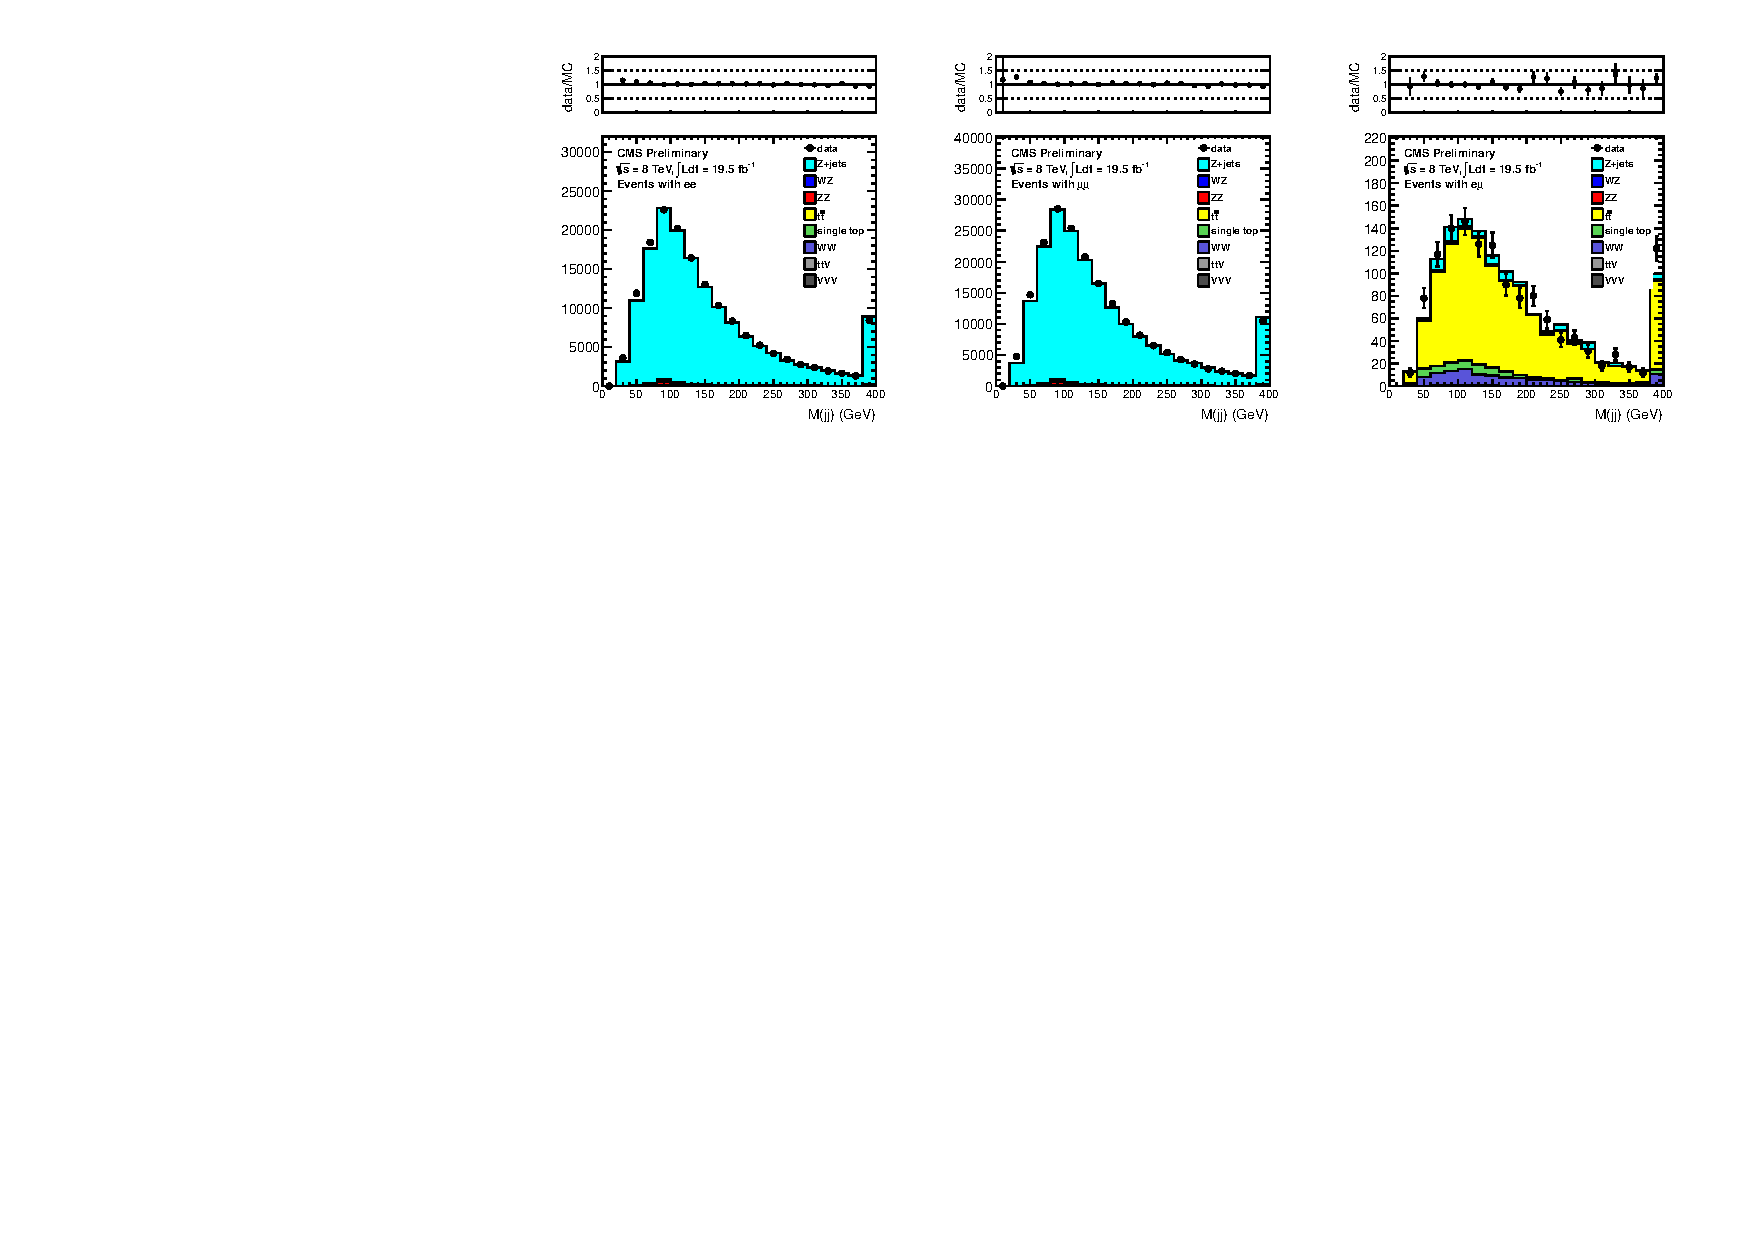
\includegraphics[width=1.0\linewidth]{plots/mjj_targeted_19p5.pdf}
	\caption{
	  \label{fig:mjj}\protect 
Distributions of dijet mass for the targeted preselection in the ee (left), $\mu\mu$ (middle) and e$\mu$ (right) final state.
}                   
  \end{center}
\end{figure}

%Loading babies at       : ../output/V00-02-13
%-------------------------------------
%USING SKIMMED SAMPLES WITH NJETS >= 2
%-------------------------------------

%Using selection         : (((((((((leptype==0 && (ee==1 || isdata==0))||(leptype==1 && (mm==1 || isdata==0)))||(leptype==2 && (em==1||me==1||isdata==0)))&&(csc==0 && hbhe==1 && hcallaser==1 && ecaltp==1 && trkfail==1 && eebadsc==1 && hbhenew==1))&&(lep1.pt()>20.0 && lep2.pt()>20.0))&&(dilmass>15.0))&&(njets>=2))&&(nbcsvm==0))&&(nlep==2))&&(dilmass>81 && dilmass<101)
%Using weight            : weight * 19.5 * trgeff * vtxweight
%Plotting var mjj flavor ee
%compareDataMC : apply trigeff 1
%MC yield VVV 13.74
%MC yield ttV 7.88
%MC yield WW 54.58
%MC yield single top 31.79
%MC yield ttbar 430.86
%MC yield ZZ 1525.36
%MC yield WZ 1454.36
%MC yield zjets 156740.32
%MC total yield 160258.89
%data yield 162621
%Plotting var mjj flavor mm
%compareDataMC : apply trigeff 1
%MC yield VVV 16.73
%MC yield ttV 9.35
%MC yield WW 66.32
%MC yield single top 37.51
%MC yield ttbar 503.49
%MC yield ZZ 1878.14
%MC yield WZ 1778.58
%MC yield zjets 196225.75
%MC total yield 200515.88
%data yield 204531
%Plotting var mjj flavor em
%compareDataMC : apply trigeff 1
%MC yield VVV 2.57
%MC yield ttV 3.16
%MC yield WW 121.17
%MC yield single top 68.54
%MC yield ttbar 1055.70
%MC yield ZZ 2.24
%MC yield WZ 13.62
%MC yield zjets 74.64
%MC total yield 1341.64
%data yield 1363


\end{comment}

\begin{figure}[!ht]
  \begin{center}
	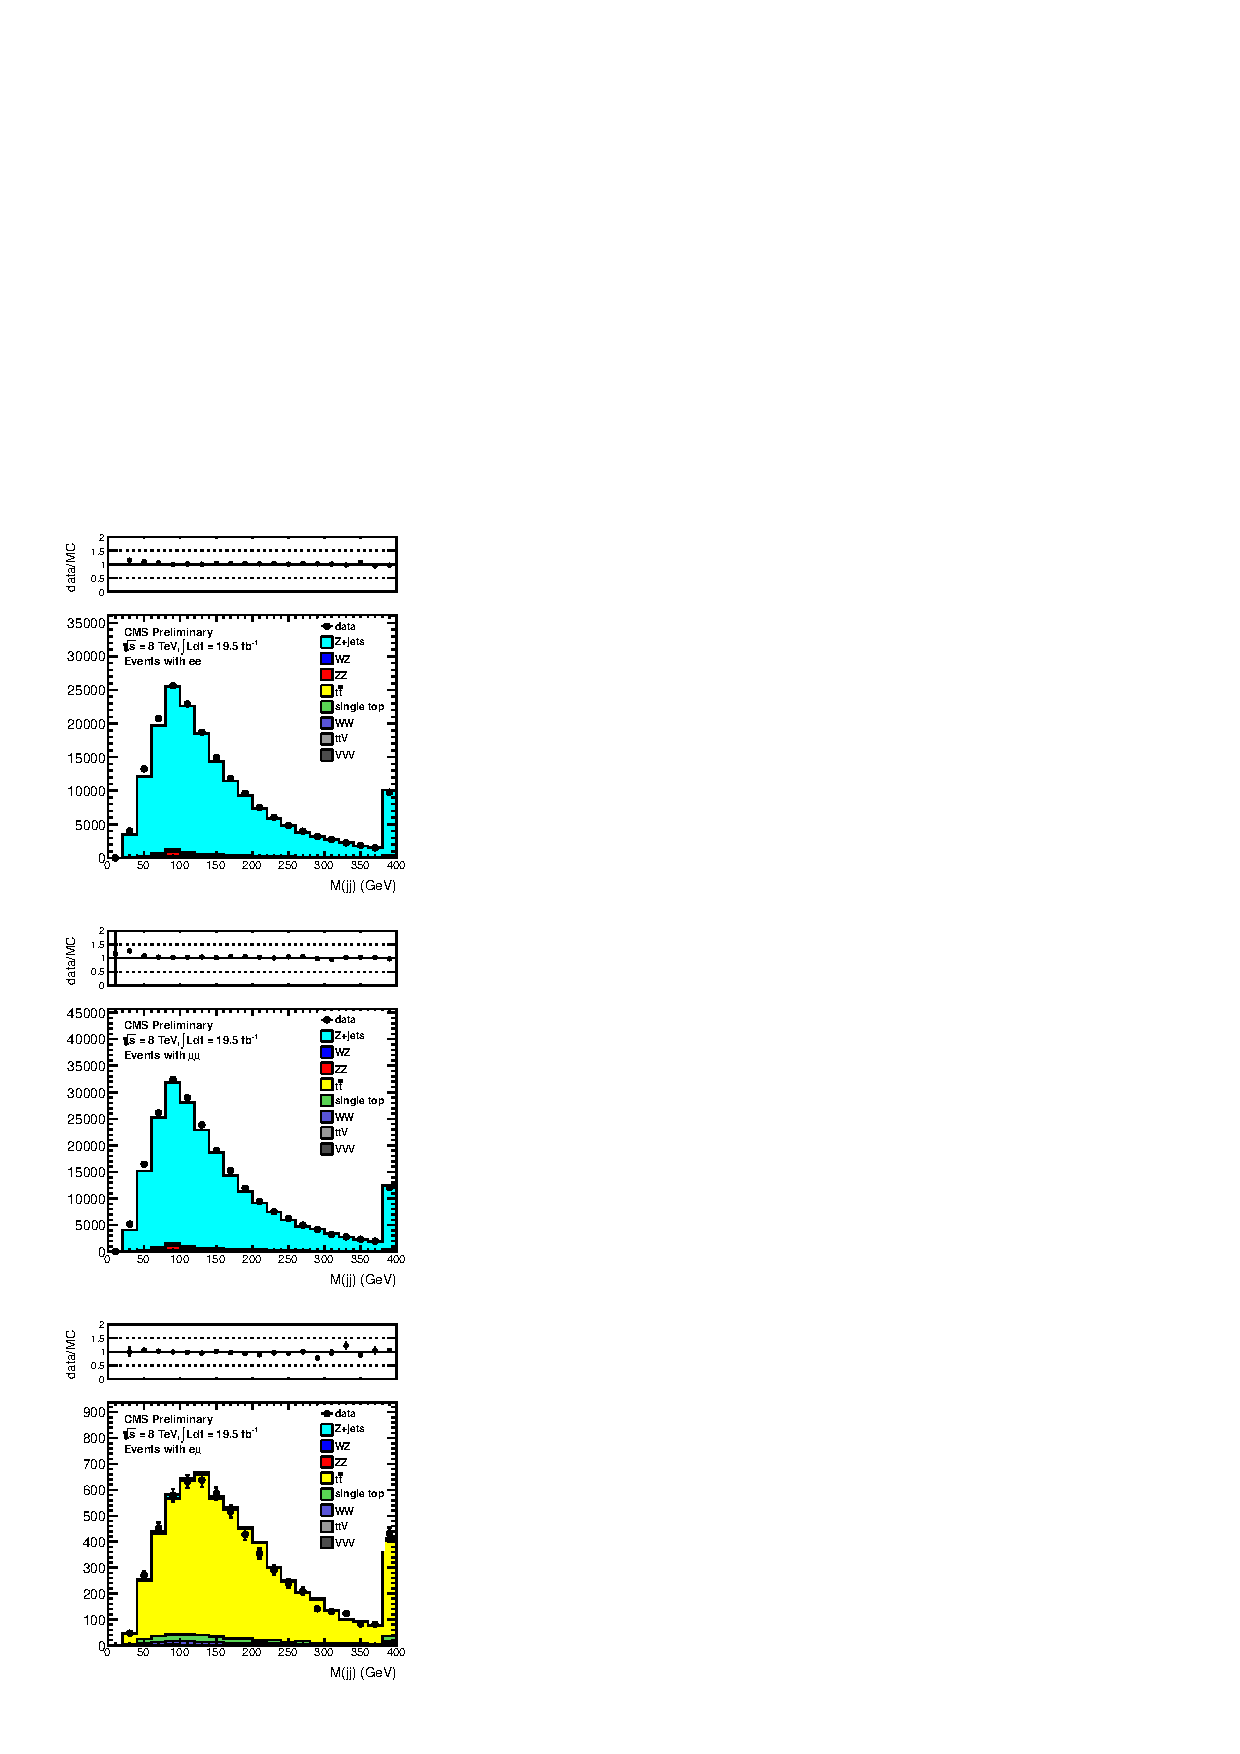
\includegraphics[width=0.35\linewidth]{plots/mjj_inclusive_19p5fb.pdf} %
	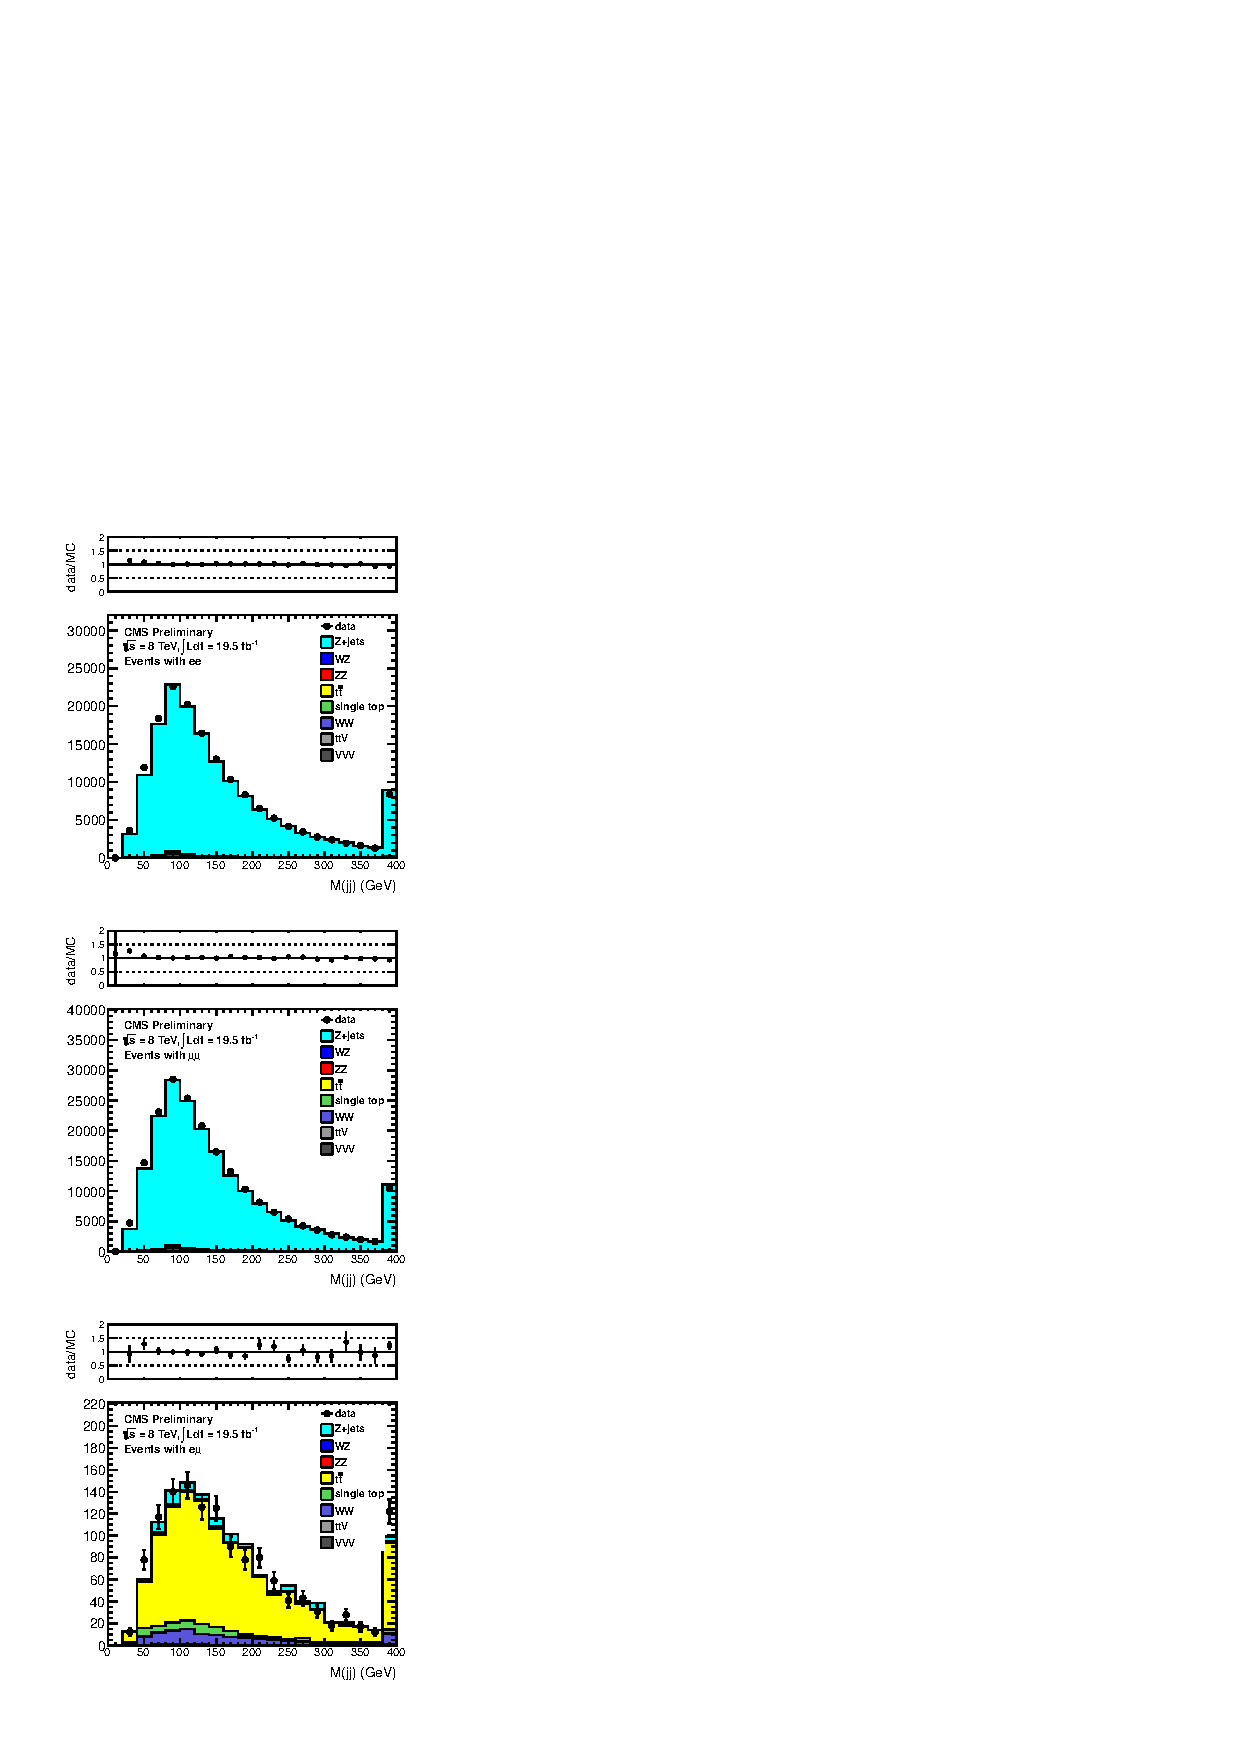
\includegraphics[width=0.35\linewidth]{plots/mjj_targeted_19p5fb.pdf}
	\caption{
	  \label{fig:mjj}\protect 
Distributions of dijet mass for the inclusive preselection (left) and targeted preselection (right), 
in the ee (top), $\mu\mu$ (middle) and e$\mu$ (bottom) final state.
}                   
  \end{center}
\end{figure}

\begin{table}[!hb]
\begin{center}
\caption{\label{table:mjj} Data and MC selection efficiencies for the dijet mass ($m_{jj}$) requirement, with respect
to the inclusive preselection.
}
\begin{tabular}{l|c|c|c}
\hline
\hline
Sample & ee & $\mu\mu$ & e$\mu$ \\
\hline
MC (inclusive)                           &180528.1 $\pm$ 646.4   &226213.8 $\pm$ 680.2   &6357.1 $\pm$ 62.7   \\
MC (inclusive + $m_{jj}$ requirement)   &48466.6 $\pm$ 333.3    &61162.1 $\pm$ 352.1   &1124.8 $\pm$ 26.5  \\
MC  efficiency  &               26.8\%  &     27.0\%  & 17.7\% \\
\hline
Data (inclusive)                           &         185555   &         234132   &           6231    \\
Data (inclusive + $m_{jj}$ requirement)   &          49256   &          62414   &           1131    \\
Data efficiency                            &          26.5\%    &       26.7\%   &            18.2\%  \\
\hline
\hline

\end{tabular}
\end{center}
\end{table}

\clearpage

\begin{figure}[!ht]
  \begin{center}
	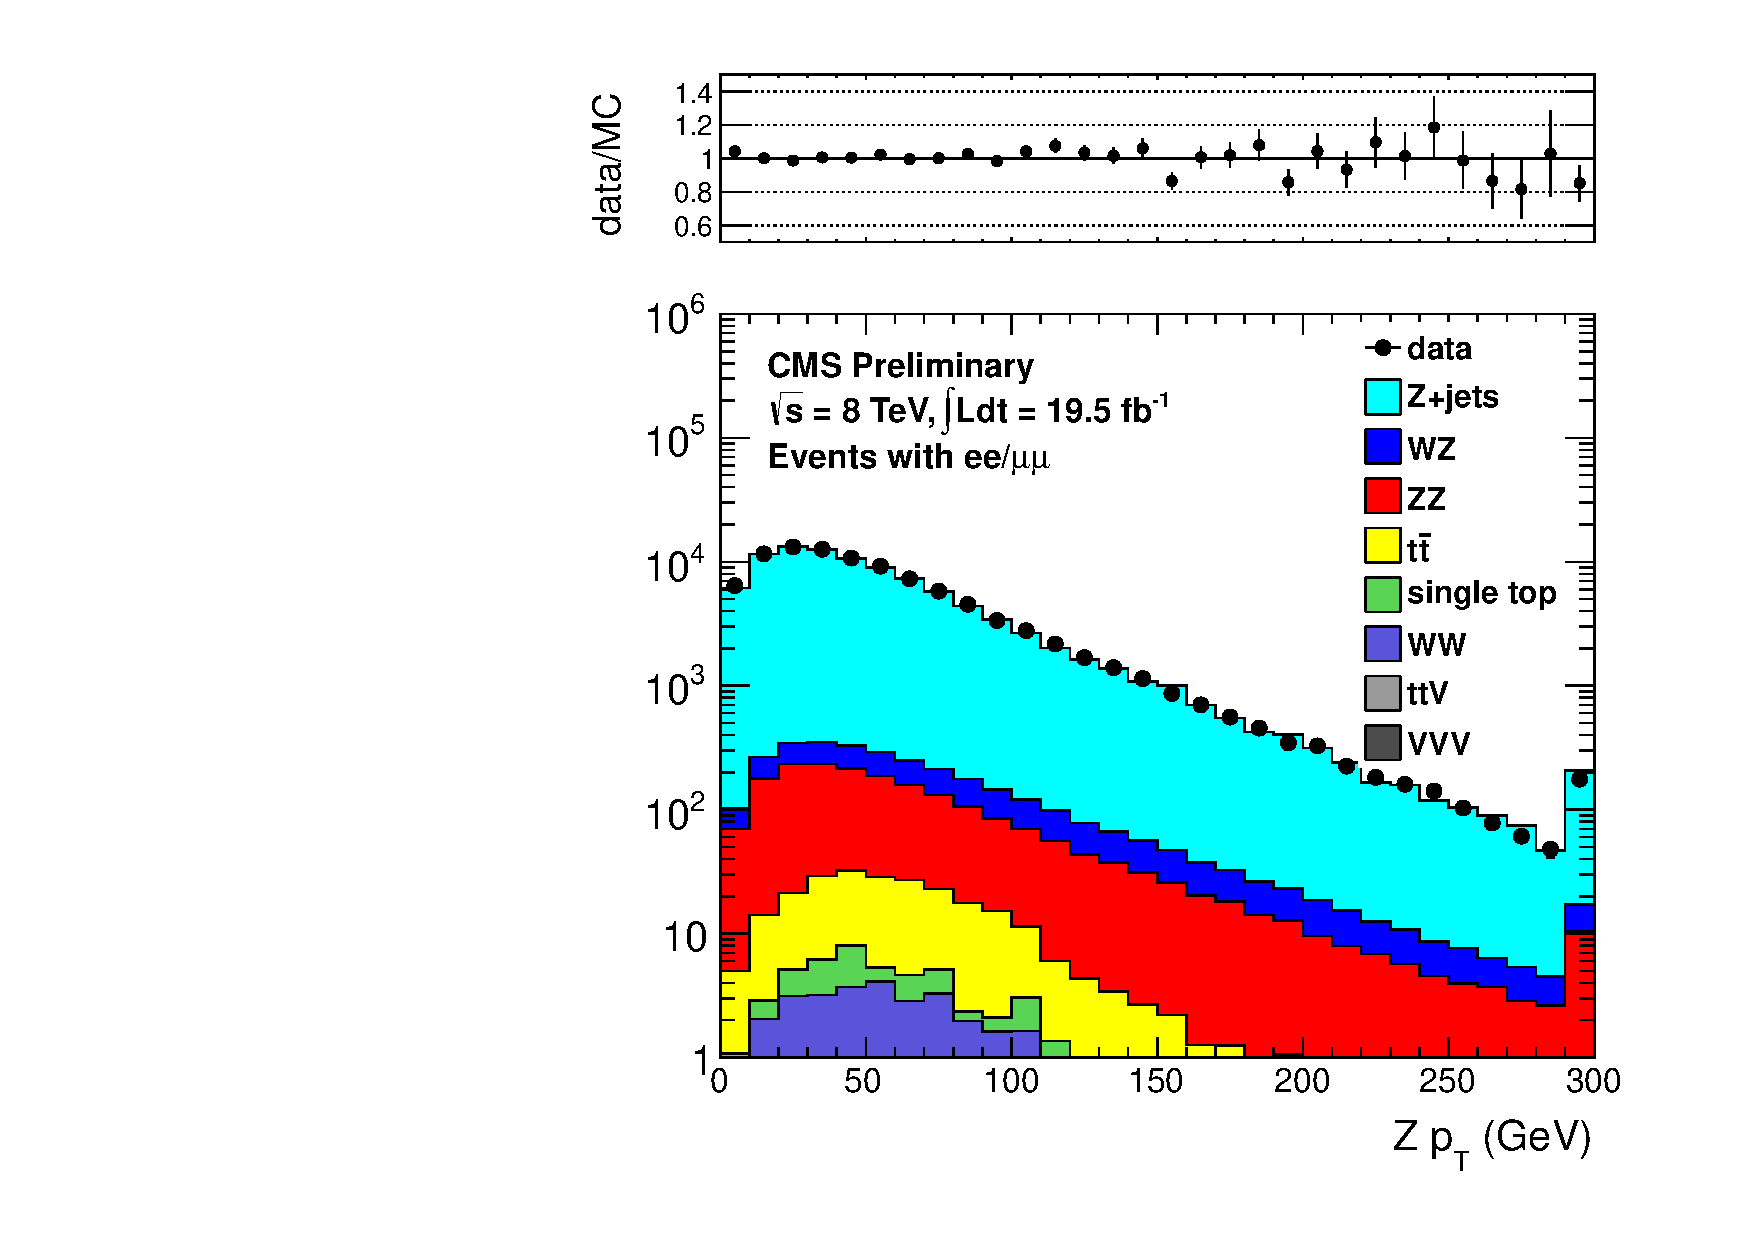
\includegraphics[width=0.45\linewidth]{plots/zpt_targeted_log.pdf}
	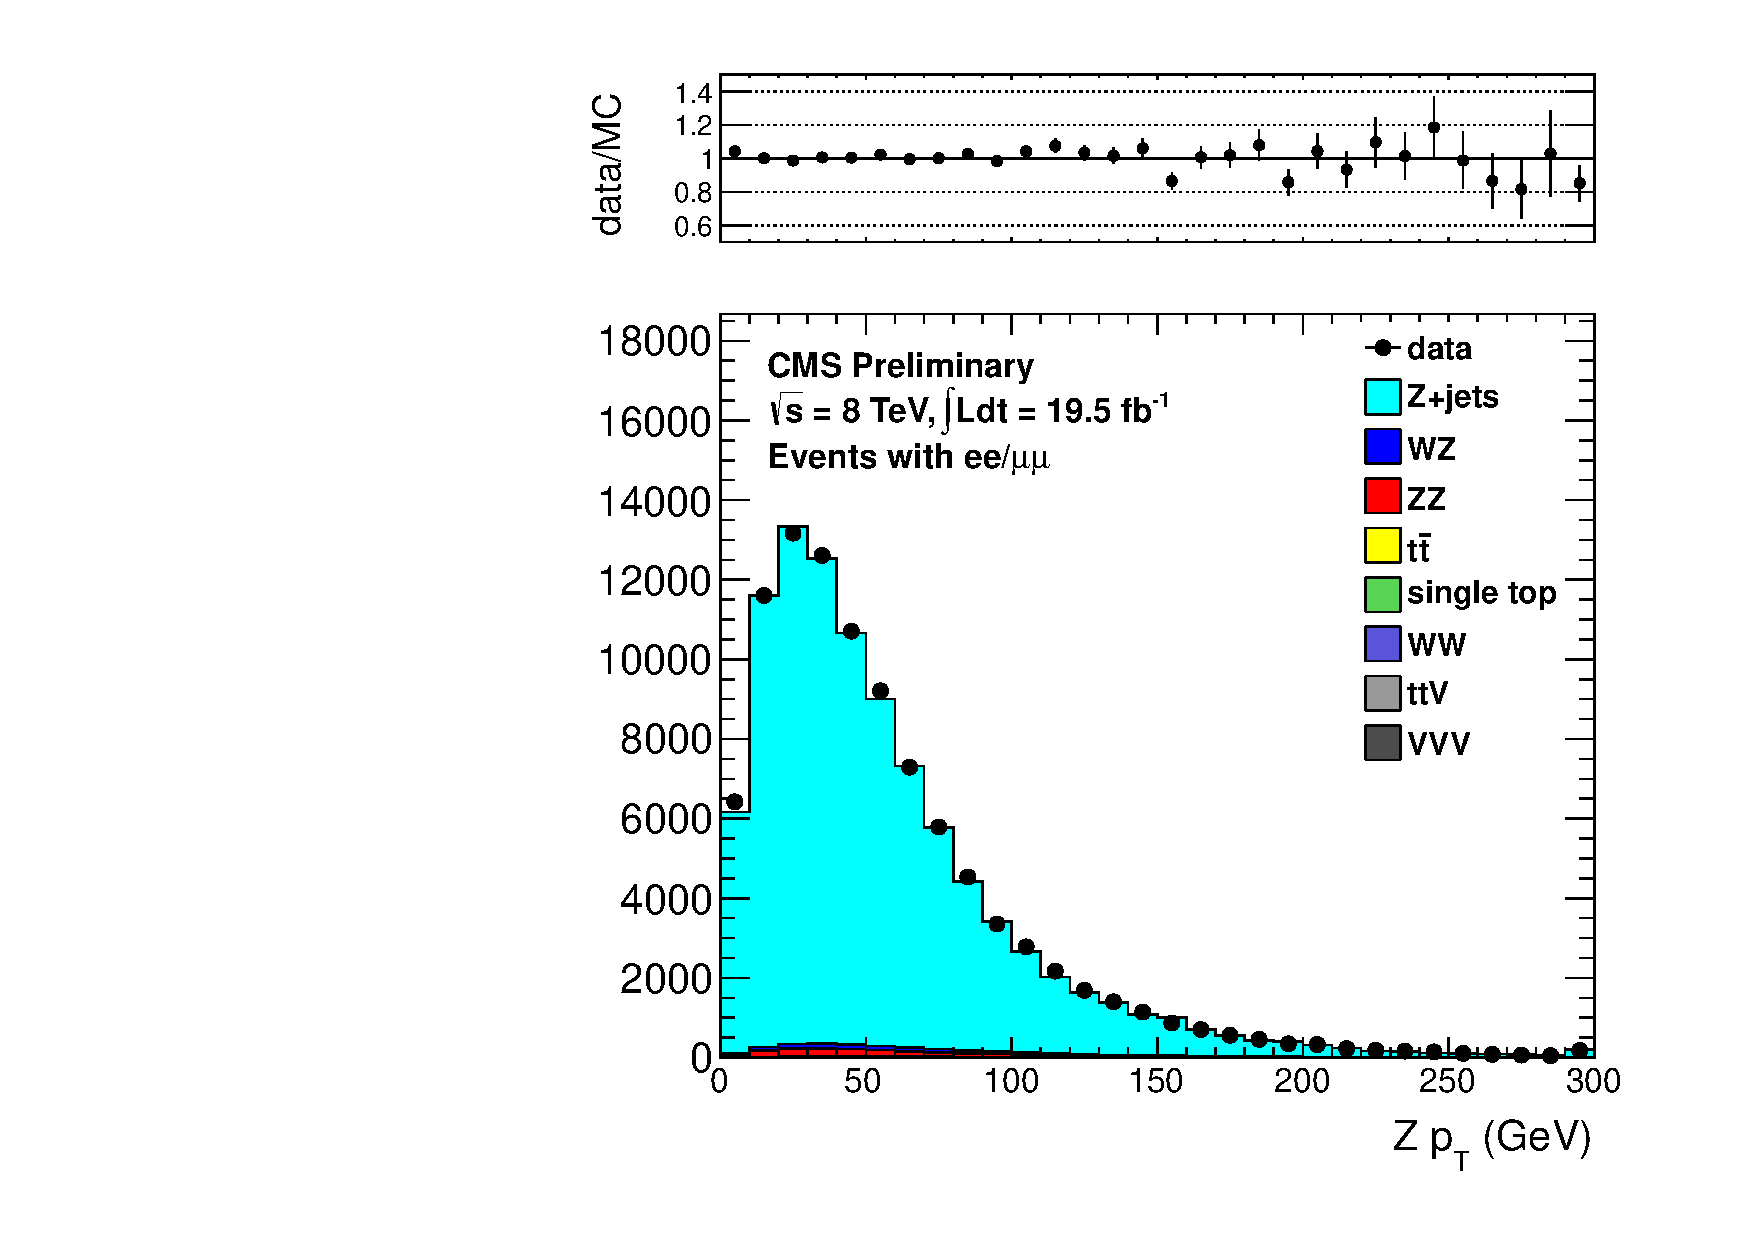
\includegraphics[width=0.45\linewidth]{plots/Zpt_targted_linear.pdf}
	\caption{
	  \label{fig:zpt}\protect 
Data/MC comparison plot of the Z \pt\ in log scale (left) and linear scale (right) for the targeted preselection.
}                   
  \end{center}
\end{figure}
